\subsection{The pbdR Project}
\makesubcontentsslidessec


\begin{frame}
  \begin{block}{Programming with Big Data in R (pbdR)}
       \centering Striving for \emph{Productivity, Portability, Performance}\\[.4cm]\pause
  \begin{columns}[onlytextwidth]
    \begin{column}{0.30\textwidth}
      \centering
       
\includegraphics[width=3.4cm]{../common/pics/simple}\\[.2cm]
    \end{column}
    \begin{column}{0.65\textwidth}
  \begin{itemize}[<+-|alert@+>]
    \item \emph{Free}\footnote{MPL, BSD, and GPL licensed} R packages.
    \item Bridging high-performance compiled code with high-productivity of R
    \item Scalable, big data analytics.
    \item Offers implicit and explicit parallelism.
    \item Methods have syntax \emph{identical} to R.
  \end{itemize}
    \end{column}
​  \end{columns}
\end{block}
\end{frame}



\begin{frame}
  \begin{block}{pbdR Packages}
    \begin{center}
%         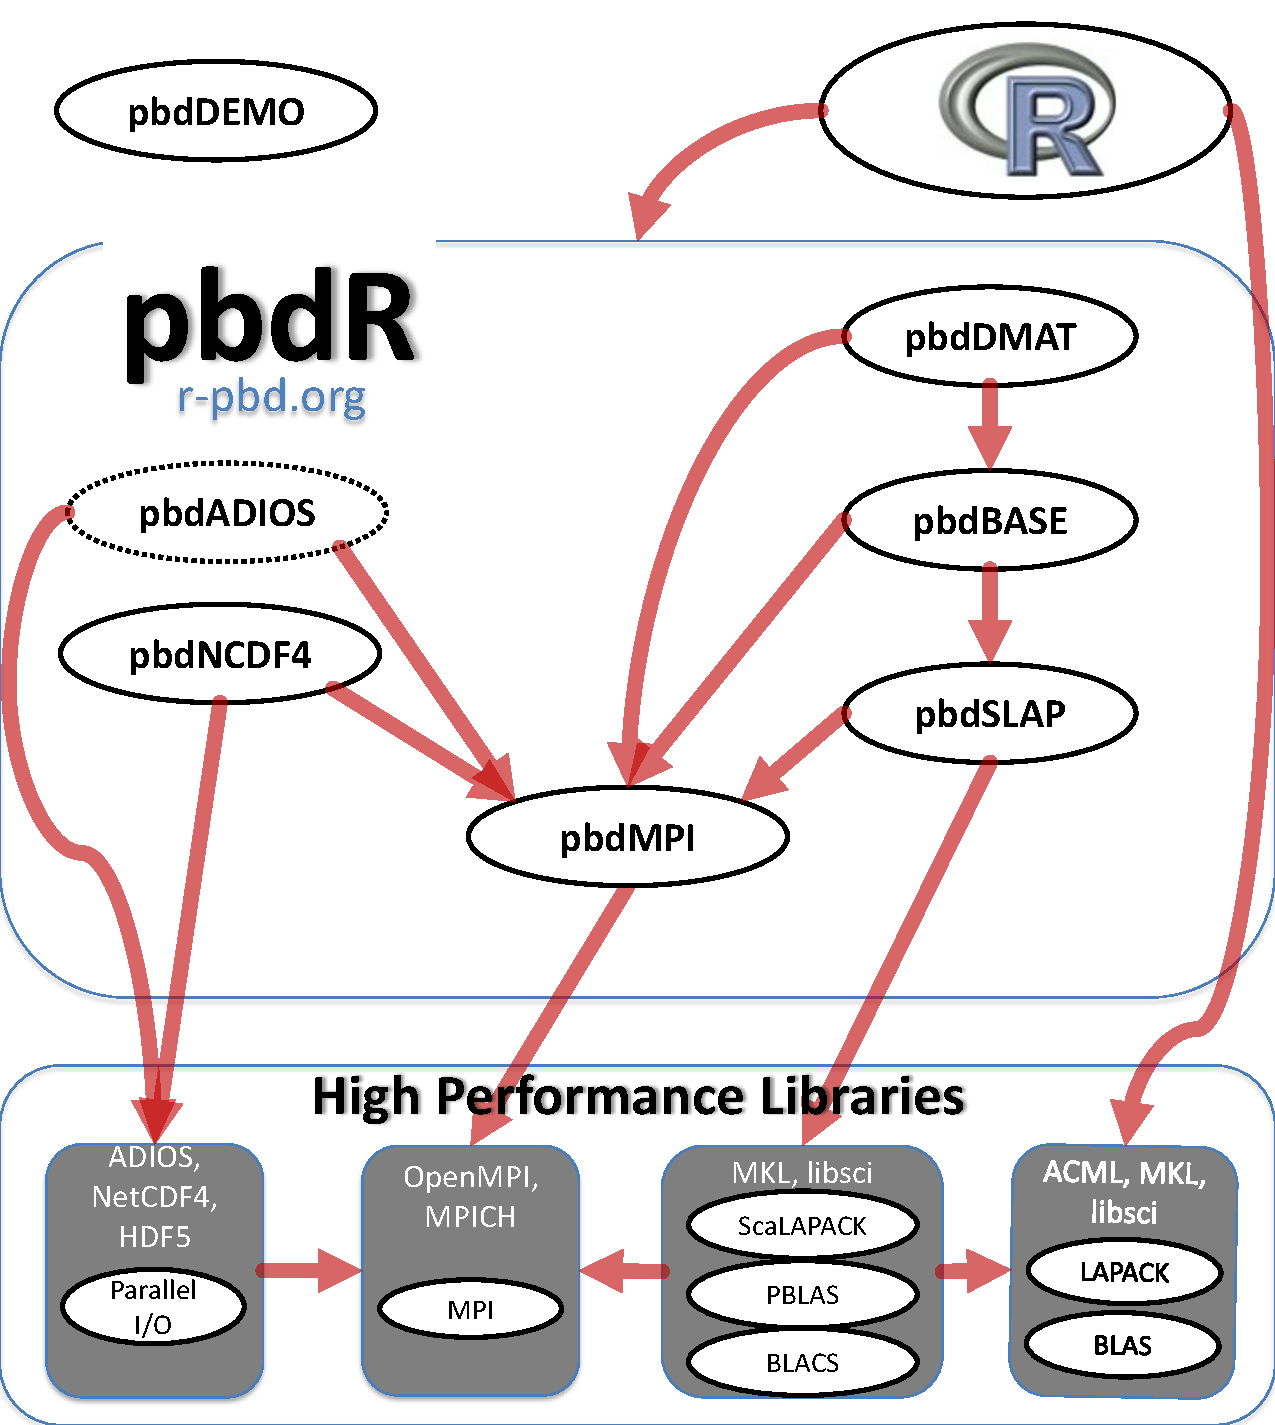
\includegraphics[width=7cm, height=7cm]{pics/pbdpacks}
      \begin{columns}
        \begin{column}{.52\textwidth}
      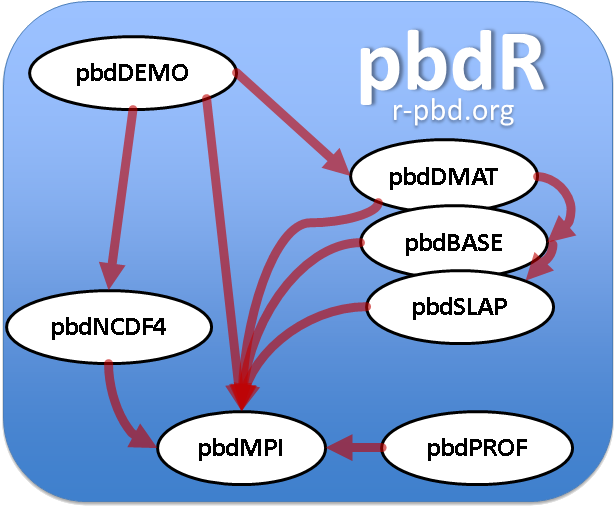
\includegraphics[scale=.4]{../common/pics/pbdR}
        \end{column}
        \hspace{.05cm}
        \begin{column}{.4\textwidth}
      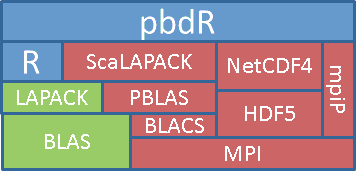
\includegraphics[scale=.45]{../common/pics/libs}
        \end{column}
      \end{columns}
    \end{center}
  \end{block}
\end{frame}


\begin{frame}
  \begin{block}{pbdR Motivation}
  Why HPC libraries (MPI, ScaLAPACK, PETSc, \dots)?
  \begin{itemize}[<+-|alert@+>]
    \item The HPC community has been at this for decades.
    \item \emph{They're tested.} \emph{They work.}  \emph{They're fast.}
    \item You're not going to beat Jack Dongarra at dense 
linear algebra.
  \end{itemize}
\end{block}
\end{frame}



%%% MPI
\begin{frame}[fragile]
  \begin{block}{Simple Interface for MPI Operations with \textbf{pbdMPI}}\pause
\begin{minipage}[t]{.475\textwidth}
\begin{lstlisting}[title=Rmpi]
# int
mpi.allreduce(x, type=1)
# double
mpi.allreduce(x, type=2)
\end{lstlisting}
\end{minipage}
\hfill
\begin{minipage}[t]{.475\textwidth}
\begin{lstlisting}[title=pbdMPI]
allreduce(x)
\end{lstlisting}
\end{minipage}
\end{block}
%
\begin{block}{Types in R}
\vspace{-.2cm}
\begin{lstlisting}
> is.integer(1)
[1] FALSE
> is.integer(2)
[1] FALSE
> is.integer(1:2)
[1] TRUE
\end{lstlisting}
\end{block}
\end{frame}




%%% DMAT/BASE/SLAP
\begin{frame}[fragile]
  \begin{block}{Distributed Matrices and Statistics with \textbf{pbdDMAT}}\pause
  \begin{center}
  \begin{minipage}{.9\textwidth}
  \centering\vspace{-.1cm}
    Matrix Exponentiation\\
\includegraphics[width=7cm,height=5.75cm]%
{../common/pics/benchmarks/expm_speedup}
  \end{minipage}
 \begin{minipage}{.9\textwidth}
 \centering
 \vspace{-.36cm}
\begin{lstlisting}
library(pbdDMAT)

dx <- ddmatrix("rnorm", 5000, 5000)
expm(dx)
\end{lstlisting}
 \end{minipage}
 \end{center}
  \end{block}
\end{frame}


\begin{frame}[fragile]
  \begin{block}{Distributed Matrices and Statistics with \textbf{pbdDMAT}}\pause
  \begin{center}
  \begin{minipage}{.9\textwidth}
  \centering\vspace{-.1cm}
	Least Squares Benchmark
		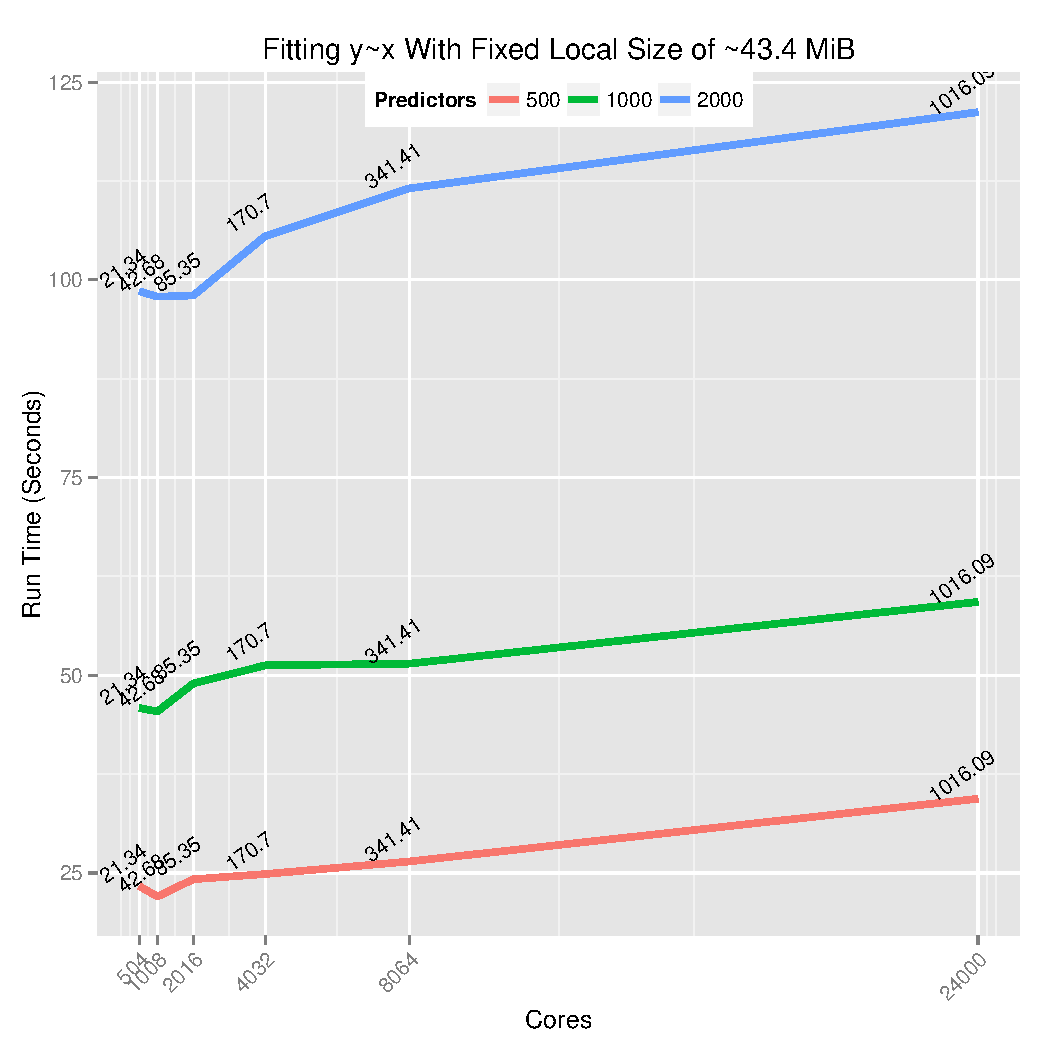
\includegraphics[width=7cm,height=5.75cm]{../common/pics/benchmarks/lmfit2}
  \end{minipage}
 \begin{minipage}{.9\textwidth}
 \vspace{-.36cm}
 \centering
\begin{lstlisting}[title=\ ,basicstyle=\scriptsize,numbers=none]
x <- ddmatrix("rnorm", nrow=m, ncol=n)
y <- ddmatrix("rnorm", nrow=m, ncol=1)
mdl <- lm.fit(x=x, y=y)
\end{lstlisting}
 \end{minipage}
 \end{center}
  \end{block}
\end{frame}


%%% DEMO
\begin{frame}[fragile]
  \begin{block}{Getting Started with HPC for R Users: \textbf{pbdDEMO}}\pause
  \begin{center}
  \begin{minipage}{.4\textwidth}
\includegraphics[width=.95\textwidth]%
{../common/pics/demo_cover.png}
  \end{minipage}
 \begin{minipage}{.58\textwidth}
    \begin{itemize}
      \item 140 page, textbook-style vignette.
      \item Over 30 demos, utilizing all$^*$ packages.
      \item Demos include:
      \begin{itemize}
        \item PCA
        \item Regression
        \item Parallel data input
        \item Model-based clustering
        \item Simple Monte Carlo simulation
        \item Bayesian MCMC
      \end{itemize}
    \end{itemize}
 \end{minipage}
 \end{center}
  \end{block}
\end{frame}